% scheme replace:
% \\scheme\{\([^\}]*\)\}
% \\scheme|\1|

%\renewcommand\chapterheadendvskip{\vspace*{5\baselineskip}}

\chapter{Programming}\label{ch:programming}\label{ch:programs}

\chapquote{The Analytical Engine has no pretensions whatever to originate any thing. It can do whatever we know how to order it to perform. It can follow analysis; but it has no power of anticipating any analytical relations or truths. Its province is to assist us in making available what we are already acquainted with.}{Augusta Ada\index{people}{Ada, Countess of Lovelace}\index{Analytical Engine}, Countess of Lovelace, in~\emph{Notes~on~the~Analytical~Engine},~1843}\index{general}{Analytical Engine}

%\chapquote{If you like programming, but you hate mathematics, don�t panic. In that case
%it�s not really mathematics you hate, it�s school. The programming you enjoy is much
%more like real mathematics than the stuff you get in most high school math classes.}{Brian Harvey~\cite{Harvey1997}}

%\renewcommand\chapterheadendvskip{\vspace*{\baselineskip}}

% This it is calculated to effect primarily and chiefly of course, through its executive faculties; but it is likely to exert an indirect and reciprocal influence on %science itself in another manner. For, in so distributing and combining the truths and the formula of analysis, that they may become most easily and rapidly amenable to %the mechanical combinations of the engine, the relations and the nature of many subjects in that science are necessarily thrown into new lights, and more profoundly 
% investigated.

What distinguishes a computer from other machines is its \emph{programmability}.  Without a program, a computer is an overpriced door stopper.  With the right program, though, a computer can be a tool for communicating across the continent, discovering a new molecule that can cure cancer, composing a symphony, or managing the logistics of a retail empire.  

Programming is the act of writing instructions that make the computer do something useful.  It is an intensely creative activity, involving aspects of art, engineering, and science.  Good programs are written to be executed efficiently by computers, but also to be read and understood by humans.  The best programs are delightful in ways similar to the best architecture, elegant in both form and function.
\sidepicture{0.12}{images/goldengate.jpg}{Golden Gate Bridge}{} % my photo

The ideal programmer would have the vision of Isaac Newton\index{people}{Newton, Isaac}, the intellect of Albert Einstein\index{people}{Einstein, Albert}, \cut{the memory of Joshua Foer, the courage of Amelia Earhart, the determination of Michael Jordan, }\cut{the pragmatism of Abraham Lincoln\index{people}{Lincoln, Abraham}, }the creativity of Miles Davis\index{people}{Davis, Miles}, the aesthetic sense of Maya Lin\index{people}{Lin, Maya}, the wisdom of Benjamin Franklin\index{people}{Franklin, Benjamin}, \cut{the foresight of Garry Kasparov\index{people}{Kasparov, Garry}, the hindsight of Edward Gibbon\index{people}{Gibbon, Edward}, }the literary talent of William Shakespeare\index{people}{Shakespeare, William}, the oratorical skills of Martin Luther King\index{people}{King, Martin Luther}, the audacity of John Roebling\index{people}{Roebling, John}, \cut{the humility of Socrates\index{people}{Socrates}, }and the self-confidence of Grace Hopper\index{people}{Hopper, Grace}.  \LATER{This list is too American.}

Fortunately, it is not necessary to possess all of those rare qualities to be a good programmer!  Indeed, anyone who is able to master the intellectual challenge of learning a language (which, presumably, anyone who has gotten this far has done at least for English) can become a good programmer.  Since programming is a new way of thinking, many people find it challenging and even frustrating at first.  Because the computer does exactly what it is told, a small mistake in a program may prevent it from working as intended.  With a bit of patience and persistence, however, the tedious parts of programming become easier, and you will be able to focus your energies on the fun and creative problem solving parts.

In the previous chapter, we explored the components of language and mechanisms for defining languages.  In this chapter, we explain why natural languages are not a satisfactory way for defining procedures and introduce a language for programming computers and how it can be used to define procedures.

\section{Problems with Natural Languages}

\index{general}{natural languages} Natural languages, such as English, work adequately (most, but certainly not all, of the time) for human-human communication, but are not well-suited for human-computer or computer-computer communication.  Why can't we use natural languages to program computers?

Next, we survey several of the reasons for this.  We use specifics from English, although all natural languages suffer from these problems to varying degrees.

\begin{list}{}{\setlength{\leftmargin}{0em}}
\item {\bf Complexity.} Although English may seem simple to you now, it took many years of intense effort (most of it subconscious) for you to learn it.  Despite using it for most of their waking hours for many years, native English speakers know a small fraction of the entire language.  The Oxford English Dictionary contains 615,000 words, of which a typical native English speaker knows about 40,000.   
\item {\bf Ambiguity.} Not only do natural languages have huge numbers of words, most words have many different meanings.  Understanding the intended meaning of an utterance requires knowing the context, and sometimes pure guesswork.  

For example, what does it mean to be paid \emph{biweekly}?  According to the American Heritage Dictionary\footnote{American Heritage, \emph{Dictionary of the English Language} (Fourth Edition), Houghton Mifflin Company, 2007 (\url{http://www.answers.com/biweekly}).}, \emph{biweekly} has two definitions:
{\em\begin{enumerate}
\item Happening every two weeks. 
\item Happening twice a week; semiweekly.
\end{enumerate}}
Merriam-Webster's Dictionary\footnote{\emph{Merriam-Webster Online}, Merriam-Webster, 2008 (\url{http://www.merriam-webster.com/dictionary/biweekly}).} takes the opposite approach:
{\em\begin{enumerate}
\item occurring twice a week   
\item occurring every two weeks : fortnightly
\end{enumerate}}
So, depending on which definition is intended, someone who is paid biweekly could either be paid once or four times every two weeks!  The behavior of a payroll management program better not depend on how biweekly is interpreted.

Even if we can agree on the definition of every word, the meaning of a sentence is often ambiguous.  This particularly difficult example is taken from the instructions with a shipment of ballistic missiles from the British Admiralty:\footnote{Carl C. Gaither and Alma E. Cavazos-Gaither, \emph{Practically Speaking: A Dictionary of Quotations on Engineering, Technology and Architecture}, Taylor \& Francis, 1998.}
\begin{quote}
{\em It is necessary for technical reasons that these warheads be stored upside down, that is, with the top at the bottom and the bottom at the top. In order that there be no doubt as to which is the bottom and which is the top, for storage purposes, it will be seen that the bottom of each warhead has been labeled 'TOP'.}
\end{quote}

\item {\bf Irregularity.}  Because natural languages evolve over time as different cultures interact and  speakers misspeak and listeners mishear, natural languages end up a morass of irregularity.  Nearly all grammar rules have exceptions.  For example, English has a rule that we can make a word plural by appending an \emph{s}.  The new word means ``more than one of the original word's meaning''.  This rule works for most words: \emph{word} $\mapsto$ \emph{words}, \emph{language} $\mapsto$ \emph{languages}, \emph{person} $\mapsto$ \emph{persons}.\footnote{Or is it \emph{people}?  What is the singular of \emph{people}? What about \emph{peeps}?  Can you only have one \emph{peep}?}  

It does not work for \emph{all} words, however.  The plural of \emph{goose} is \emph{geese} (and \emph{gooses} is not an English word), the plural of \emph{deer} is \emph{deer} (and \emph{deers} is not an English word), and the plural of \emph{beer} is controversial (and may depend on whether you speak American English or Canadian English).
%\footnote{See http://crofsblogs.typepad.com/english/2005/06/beer\_or\_beers.html.}).  

These irregularities can be charming for a natural language, but they are a constant source of difficulty for non-native speakers attempting to learn a language.  There is no sure way to predict when the rule can be applied, and it is necessary to memorize each of the irregular forms.

\item {\bf Uneconomic.}  \marginquote{I have made this letter longer than usual, only because I have not had the time to make it shorter.}{Blaise Pascal, 1657}\index{people}{Pascal, Blaise}It requires a lot of space to express a complex idea in a natural language.  Many superfluous words are needed for grammatical correctness, even though they do not contribute to the desired meaning.  Since natural languages evolved for everyday communication, they are not well suited to describing the precise steps and decisions needed in a computer program.  
\LATER{Faulkner quote - poet -> short story writer -> novelist}

As an example, consider a procedure for finding the maximum of two numbers.  In English, we could describe it like this:
\begin{quote}
{\em To find the maximum of two numbers, compare them.  If the first number is greater than the second number, the maximum is the first number.  Otherwise, the maximum is the second number.}
\end{quote}
Perhaps shorter descriptions are possible, but any much shorter description probably assumes the reader already knows a lot.  By contrast, we can express the same steps in the Scheme programming language in very concise way (don't worry if this doesn't make sense yet---it should by the end of this chapter): 
\begin{schemedisplay}
     (define (bigger a b) (if (> a b) a b))
\end{schemedisplay}

\begin{comment}
\begin{pythoncode}
def bigger(a,b):
	if (a > b): return a
	else: return b
\end{pythoncode}
\end{comment}

\item {\bf Limited means of abstraction.}\index{general}{means of abstraction}  Natural languages provide small, fixed sets of pronouns to use as means of abstraction, and the rules for binding pronouns to meanings are often unclear.  \cut{As discussed in Section~\ref{sec:language-construction}, the means of abstraction available in English are particularly poor. } Since programming often involves using simple names to refer to complex things, we need more powerful means of abstraction than natural languages provide.   

\end{list}

\section{Programming Languages}

For programming computers, we want simple, unambiguous, regular, and economical languages with powerful means of abstraction.  A \definition{programming language} is a language that is designed to be read and written by humans to create programs that can be executed by computers.
%\footnote{We will provide a more precise definition of \emph{programming language} in Chapter~\ref{ch-models}, after we have a formal model of a computer.} 

Programming languages come in many flavors.  It is difficult to simultaneously satisfy all desired properties since simplicity is often at odds with economy.  Every feature that is added to a language to increase its expressiveness incurs a cost in reducing simplicity and regularity.  For the first two parts of this book, we use the Scheme programming language which was designed primarily for simplicity.  For the later parts of the book, we use the Python programming language, which provides more expressiveness but at the cost of some added complexity.

Another reason there are many different programming languages is that they are at different \emph{levels of abstraction}\index{general}{abstraction}.  Some languages provide programmers with detailed control over machine resources, such as selecting a particular location in memory where a value is stored.  Other languages hide most of the details of the machine operation from the programmer, allowing them to focus on higher-level actions.

Ultimately, we want a program the computer can execute.  This means at the lowest level we need languages the computer can understand directly.  At this level, the program is just a sequence of bits encoding machine instructions.  Code at this level is not easy for humans to understand or write, but it is easy for a processor to execute quickly.  The machine code encodes instructions that direct the processor to take simple actions like moving data from one place to another, performing simple arithmetic, and jumping around to find the next instruction to execute.\index{general}{machine code}

For example, the bit sequence \textsf{1110101111111110} encodes an instruction in the Intel x86 instruction set (used on most PCs) that instructs the processor to jump backwards two locations.  Since the instruction itself requires two locations of space, jumping back two locations actually jumps back to the beginning of this instruction.  Hence, the processor gets stuck running forever without making any progress.  

\sidepicture{0.20}{images/1952_hopper-grace_large-1.jpg}{Grace Hopper}{Image courtesy Computer History Museum (1952)} \index{people}{Hopper, Grace}
The computer's processor is designed to execute very simple instructions like jumping, adding two small numbers, or comparing two values.  This means each instruction can be executed very quickly.  A typical modern processor can execute \emph{billions} of instructions in a second.\footnote{A ``2GHz processor'' executes 2 billion cycles per second.  This does not map directly to the number of instructions it can execute in a second, though, since some instructions take several cycles to execute.}  

Until the early 1950s, all programming was done at the level of simple instructions.   The problem with instructions at this level is that they are not easy for humans to write and understand, and you need many simple instructions before you have a useful program. 

A \definition{compiler} is a computer program that generates other programs.  It translates an input program written in a \emph{high-level language} that is easier for humans to create into a program in a machine-level language that can be executed by the computer.  Admiral Grace Hopper developed the first compilers in the 1950s.  
% http://www.computerhistory.org/timeline/images/1952_hopper-grace_large.jpg - need permission for commercial use http://www.computerhistory.org/terms/

An alternative to a compiler is an interpreter.  An \definition{interpreter} is a tool that translates between a higher-level language and a lower-level language, but where a compiler translates an entire program at once and produces a machine language program that can be executed directly, an interpreter interprets the program a small piece at a time while it is running.  \marginquote{Nobody believed that I had a running compiler and nobody would touch it. They told me computers could only do arithmetic.}{Grace Hopper} This has the advantage that we do not have to run a separate tool to compile a program before running it; we can simply enter our program into the interpreter and run it right away.  This makes it easy to make small changes to a program and try it again, and to observe the state of our program as it is running. 

One disadvantage of using an interpreter instead of a compiler is that because the translation is happening while the program is running, the program executes slower than a compiled program.  Another advantage of compilers over interpreters is that since the compiler translates the entire program it can also analyze the program for consistency and detect certain types of programming mistakes automatically instead of encountering them when the program is running (or worse, not detecting them at all and producing unintended results).  This is especially important when writing critical programs such as flight control software --- we want to detect as many problems as possible in the flight control software before the plane is flying!  

Since we are more concerned with interactive exploration than with performance and detecting errors early, we use an interpreter instead of a compiler.  

\section{Scheme}\index{general}{Scheme}

The programming system we use for the first part of this book is depicted in Figure~\ref{fig:scheme-programming}.   The input to our programming system is a program written in a programming language named \emph{Scheme}.  A Scheme interpreter interprets a Scheme program and executes it on the machine processor.

\begin{figure}[!b]
\begin{center}
% image in picture from: http://en.wikipedia.org/wiki/File:80486dx2-large.jpg
\vspace*{2.0ex}

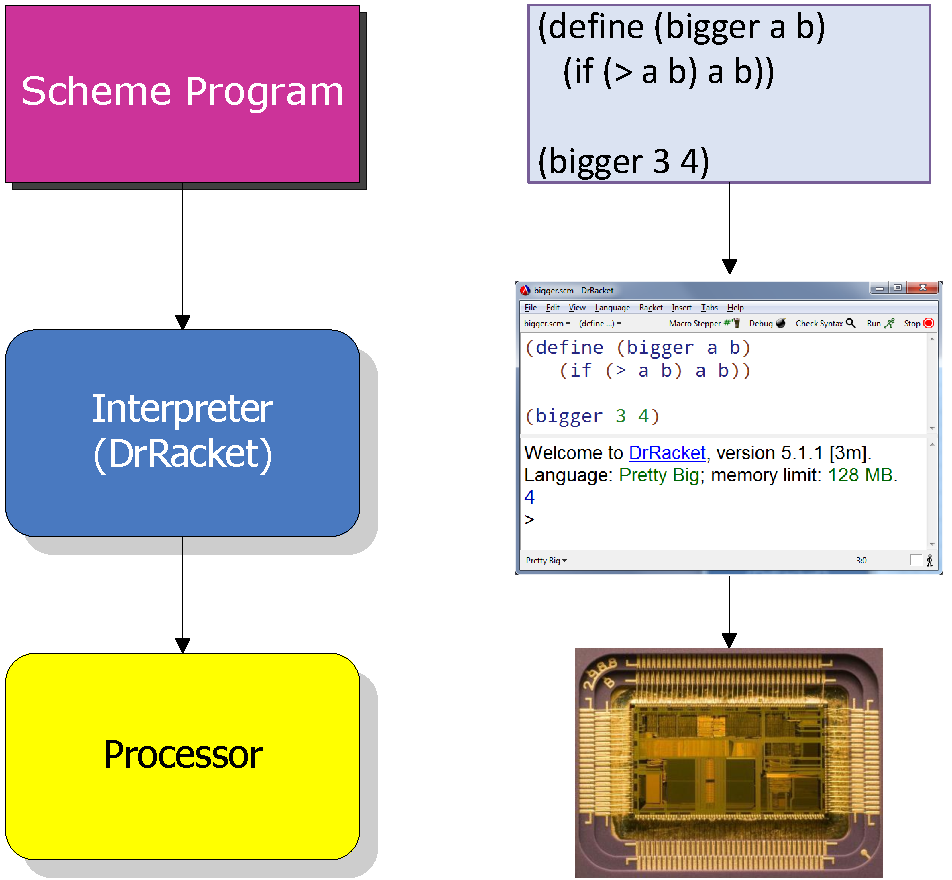
\includegraphics[height=3.0in]{figures/languagesystem.pdf}
\caption{Running a Scheme program.\label{fig:scheme-programming}}
\end{center}
\end{figure}

Scheme was developed at MIT in the 1970s by Guy Steele\index{people}{Steele, Guy} and Gerald Sussman\index{people}{Sussman, Gerald}, based on the LISP\index{general}{LISP} programming language that was developed by John McCarthy\index{people}{McCarthy, John} in the 1950s.  
\cut{\footnote{Originally, it was named ``Schemer'', but the machine used to develop it only supported 6-letter file names, so the name was shortened to ``Scheme''.} }
Although many large systems have been built using Scheme, it is not widely used in industry.  It is, however, a great language for learning about computing and programming.  The primary advantage of using Scheme to learn about computing is its simplicity and elegance.  The language is simple enough that this chapter covers nearly the entire language (we defer describing a few aspects until Chapter~\ref{ch:state}), and by the end of this book you will know enough to implement your own Scheme interpreter.  By contrast, some programming languages that are widely used in industrial programming such as C++ and Java require thousands of pages to describe, and even the world's experts in those languages do not agree on exactly what all programs mean.  

Although almost everything we describe should work in all Scheme interpreters, for the examples in this book we assume the DrRacket\index{general}{DrRacket} programming environment which is freely available from \url{http://racket-lang.org/}.  DrRacket includes interpreters for many different languages, so you must select the desired language using the \keyword{Language} menu.  The selected language defines the grammar and evaluation rules that will be used to interpret your program.  For all the examples in this book, we use a version of the Scheme language named \keyword{Pretty Big}.  

\section{Expressions}\label{sec:expressions}

A Scheme program is composed of expressions and definitions (we cover definitions in Section~\ref{sec:definitions}).  An \definition{expression} is a syntactic element that has a \emph{value}.  

The act of determining the value associated with an expression is called \definition{evaluation}.  A Scheme interpreter, such as the one provided in DrRacket, is a machine for evaluating Scheme expressions.  If you enter an expression into a Scheme interpreter, the interpreter evaluates the expression and displays its value.

Expressions may be primitives.  Scheme also provides means of combination for producing complex expressions from simple expressions.  The next subsections describe primitive expressions and application expressions.  Section~\ref{sec:procedures} describes expressions for making procedures and Section~\ref{sec:decisions} describes expressions that can be used to make decisions.

\subsection{Primitives}\label{sec:primitives}\index{general}{primitive expressions}

An expression can be replaced with a primitive:
\begin{bnfgrammarm}{Expression}
\bnfrule{Expression}{\nonterminal{PrimitiveExpression}}
\end{bnfgrammarm}
As with natural languages, primitives are the smallest units of meaning.  Hence, the value of a primitive is its pre-defined meaning.  

Scheme provides many different primitives.  Three useful types of primitives are described next: numbers, Booleans, and primitive procedures.

\shortsection{Numbers}\index{general}{numbers} Numbers represent numerical values.  Scheme provides all the kinds of numbers you are familiar with including whole numbers, negative numbers, decimals, and rational numbers.\cut{, and they mean almost exactly what you think they mean.\footnote{The details of representing numbers on computers are complex, and we do not consider them here.}}

Example numbers include:
\begin{smallquote}
\begin{tabbing}
\scheme|3.14159| \qquad \= \scheme|3/4| \quad \= \kill
\scheme|150| \> \scheme|0| \> \scheme|-12| \\
\scheme|3.14159| \> \scheme|3/4| \> \scheme|999999999999999999999|\\
\end{tabbing}
\end{smallquote}
Numbers evaluate to their value.  For example, the value of the primitive expression \scheme|1120| is \schemeresult|1120|.
%\begin{schemeregion}
%\sidenote{By convention, we use \sl{\schemeresult{slanted}} font to show values.}
%\end{schemeregion}

%\TODO{Explain typesetting conventions.  In the DrRacket interactions window, values are shown in blue.}

\shortsection{Booleans} \index{general}{Boolean} Booleans represent truth values.  There are two primitives for representing true and false:
\begin{bnfgrammarm}{PrimitiveExpression}
\bnfrule{PrimitiveExpression}{\scheme|true| $\mid$ \scheme|false|}
\end{bnfgrammarm}
The meaning of \scheme|true| is true, and the meaning of \scheme|false| is false.  In the DrRacket interpreter, \scheme|#t| and \scheme|#f| are used to represent the primitive truth values.  So, the value \scheme|true| appears as \scheme|#t| in the interactions window.

\index{general}{primitive procedures}
\shortsection{Primitive Procedures}\label{built-in-procs} Scheme provides primitive procedures corresponding to many common functions.  Mathematically, a \definition{function} is a mapping from inputs to outputs.  For each valid input to the function, there is exactly one associated output.  For example, \scheme|+| is a procedure that takes zero or more inputs, each of which must be a number.  Its output is the sum of the values of the inputs.  Table \ref{scheme-funcs} describes some primitive procedures for performing arithmetic and comparisons on numbers.


\begin{table}[!t]\index{general}{primitive procedures}
\centering \small \raggedright
\begin{tabular}{cp{1.0in}p{1.0in}p{2.0in}} %\hline
{\bfseries Symbol} & \multicolumn{1}{c}{\bfseries Description} & \multicolumn{1}{c}{\bfseries Inputs} & \multicolumn{1}{c}{\bfseries Output} \tabularnewline[6pt] % \hline 
% \hline \multicolumn{4}{|c|}{Arithmetic} \tabularnewline  \hline
	\scheme|+|  & add & \raggedright zero or more numbers & \raggedright	sum of the input numbers (\schemeresult|0| if there are no inputs) \tabularnewline[6pt]  
\scheme|*|  & multiply & \raggedright zero or more numbers & \raggedright product of the input numbers (\schemeresult|1| if there are no inputs) \tabularnewline[6pt]
 \scheme|-|	& subtract & \raggedright two numbers	& \raggedright the value of the first number minus the value the second number \tabularnewline[6pt] 
 \scheme|/|  & divide & \raggedright two numbers & \raggedright the value of the first number divided by the value of the second number \tabularnewline[12pt] % \hline
% \hline \multicolumn{4}{|c|}{Comparison} \tabularnewline  \hline
\scheme|zero?| & \raggedright is zero? & \raggedright one number & \raggedright \schemeresult|true| if the input value is \scheme|0|, otherwise \schemeresult|false|
\tabularnewline[6pt] 
\scheme|=|	& \raggedright is equal to? & \raggedright two numbers & \raggedright \schemeresult|true| if the input values have the same value, otherwise \schemeresult|false| \tabularnewline[6pt] 
\scheme|<|  & \raggedright is less than? & \raggedright two numbers & \raggedright \schemeresult|true| if the first input value has lesser value than the second input value, otherwise \schemeresult|false| \tabularnewline[6pt] 
\scheme|>|  & \raggedright is greater than? & \raggedright two numbers & \raggedright \schemeresult|true| if the first input value has greater value than the second input value, otherwise \schemeresult|false| \tabularnewline[6pt] 
\scheme|<=| & \raggedright is less than or equal to?& \raggedright two numbers & \raggedright \schemeresult|true| if the first input value is not greater than the second input value, otherwise \schemeresult|false| \tabularnewline[6pt] 
\scheme|>=| & \raggedright is greater than or equal to? & \raggedright two numbers & \raggedright \schemeresult|true| if the first input value is not less than the second input value, otherwise \schemeresult|false| \tabularnewline[12pt] %  \hline
\end{tabular} \\[0.5ex]
\caption{\label{scheme-funcs} Selected Scheme Primitive Procedures.} 
\subcap{All of these primitive procedures operate on numbers.  The first four are the basic arithmetic operators; the rest are comparison procedures.  Some of these procedures are defined for more inputs than just the ones shown here (e.g., the subtract procedure also works on one number, producing its negation).}
\end{table}

\subsection{Application Expressions}\label{sec:application}

Most of the actual work done by a Scheme program is done by \emph{application expressions} that apply procedures to operands.  The expression \scheme|(+ 1 2)| is an \nonterminal{ApplicationExpression}, consisting of three subexpressions.  Although this example is probably simple enough that you can probably guess that it evaluates to \tb{\schemeresult|3|}, we will show in detail how it is evaluated by breaking down into its subexpressions using the grammar rules.  The same process will allow us to understand how \emph{any} expression is evaluated.

The grammar rule for application is:
\begin{schemeregion}
\begin{bnfgrammarm}{ApplicationExpression}
\bnfrule{Expression}{\nonterminal{ApplicationExpression}}
\bnfrule{ApplicationExpression}{\scheme|(|\nonterminal{Expression} \nonterminal{MoreExpressions}\scheme|)|}
\bnfrule{MoreExpressions}{$\epsilon$ $\mid$ \nonterminal{Expression} \nonterminal{MoreExpressions}}
\end{bnfgrammarm}
\end{schemeregion}
This rule produces a list of one or more expressions surrounded by parentheses.  The value of the first expression should be a procedure; \cut{.  All of the primitive procedures are procedures; in Section~\ref{sec:procedures}, we will see how to create new procedures.  T} the remaining expressions are the inputs to the procedure known as \definition{operands}.  Another name for operands is \definition{arguments}.  

Here is a parse tree for the expression \scheme|(+ 1 2)|:
\begin{center}\small
\Treek[1]{1.5}{ & & \K{\nonterminal{Expression}} \B{d} \\
       & & \K{\nonterminal{ApplicationExpression}} \B{dll} \B{dl} \B{drr} \B{drrrrr} \\ 
       \K[-4]{\scheme|(|} & \K[-1]{\nonterminal{Expression}} \B{d} & & & \K[0]{\nonterminal{MoreExpressions}} \B{dl} \B{drr} & & & \K[4]{\scheme|)|} \\ 
                              & \K[-5]{\nonterminal{PrimitiveExpression}} \B{d} & & \K{\nonterminal{Expression}} \B{d} & & &\K[-2]{\nonterminal{MoreExpressions}} \B{dl} \B{dr} \\
                              & \K{\scheme|+|}                            & & \K{\nonterminal{PrimitiveExpression}} \B{d} & & \K{\nonterminal{Expression}} \B{d} & & \K[1]{\nonterminal{MoreExpressions}} \B{d} \\
                              & 								                            & & \K{\scheme|1|}                            & & \K{\nonterminal{PrimitiveExpression}} \B{d} & & \K{$\epsilon$} \\
                              &                                             & &                                             & & \K{\scheme|2|} 
}
\end{center}

Following the grammar rules, we replace \nonterminal{Expression} with \nonterminal{ApplicationExpression} at the top of the parse tree.  Then, we replace \nonterminal{ApplicationExpression} with {\scheme|(|\nonterminal{Expression} \nonterminal{MoreExpressions}\scheme|)|}.  The \nonterminal{Expression} term is replaced \nonterminal{PrimitiveExpression}, and finally, the primitive addition procedure \scheme|+|.  This is the first subexpression of the application, so it is the procedure to be applied.  The \nonterminal{MoreExpressions} term produces the two operand expressions: \scheme|1| and \scheme|2|, both of which are primitives that evaluate to their own values.  The application expression is evaluated by applying the value of the first expression (the primitive procedure \scheme|+|) to the inputs given by the values of the other expressions.  Following the meaning of the primitive procedure, \scheme|(+ 1 2)| evaluates to \tb{\schemeresult|3|} as expected.

The \nonterminal{Expression} nonterminals in the application expression can be replaced with anything that appears on the right side of an expression rule, including an \nonterminal{ApplicationExpression}.  

We can build up complex expressions like \scheme|(+ (* 10 10) (+ 25 25))|. Its parse tree is:

\begin{center}\small
\Treek[1]{1.5}{ & & \K{\nonterminal{Expression}} \B{d} \\
       & & \K{\nonterminal{ApplicationExpression}} \B{dll} \B{dl} \B{drr} \B{drrrrr} \\ 
       \K[-4]{\scheme|(|} & \K[-1]{\nonterminal{Expression}} \B{d} & & & \K[0]{\nonterminal{MoreExpressions}} \B{dl} \B{drr} & & & \K[4]{\scheme|)|} \\ 
                              & \K[-5]{\nonterminal{PrimitiveExpression}} \B{d} & & \K{\nonterminal{Expression}} \B{d} & & &\K{\nonterminal{MoreExpressions}} \B{dl} \B{dr} \\
                              & \K{\scheme|+|}                            & & \K[-2]{\nonterminal{ApplicationExpression}} \TRi & & \K[2]{\nonterminal{Expression}} \B{d} & & \K[-4]{\nonterminal{MoreExpressions}} \B{d} \\
                              & 								                            & & \K{\scheme|(* 10 10)|}                            & & \K[4]{\nonterminal{ApplicationExpression}} \TRi & & \K{$\epsilon$} \\
                              &                                             & &                                             & & \K{\scheme|(+ 25 25)|}}
\end{center}
This tree is similar to the previous tree, except instead of the subexpressions of the first application expression being simple primitive expressions, they are now application expressions.  (Instead of showing the complete parse tree for the nested application expressions, we use triangles.)

To evaluate the output application, we need to evaluate all the subexpressions.  The first subexpression, \scheme|+|, evaluates to the primitive procedure.  The second subexpression, \scheme|(* 10 10)|, evaluates to \tb{\schemeresult|100|}, and the third expression, \scheme|(+ 25 25)|, evaluates to \tb{\schemeresult|50|}.  Now, we can evaluate the original expression using the values for its three component subexpressions: \scheme|(+ 100 50)| evaluates to \tb{\schemeresult|150|}.

\begin{schemeregion}

\beforeex
\begin{exercise}
Draw a parse tree for the Scheme expression \scheme|(+ 100 (* 5 (+ 5 5)))| and show how it is evaluated.
\solution{
The full parse tree for the expression is:
\begin{center}
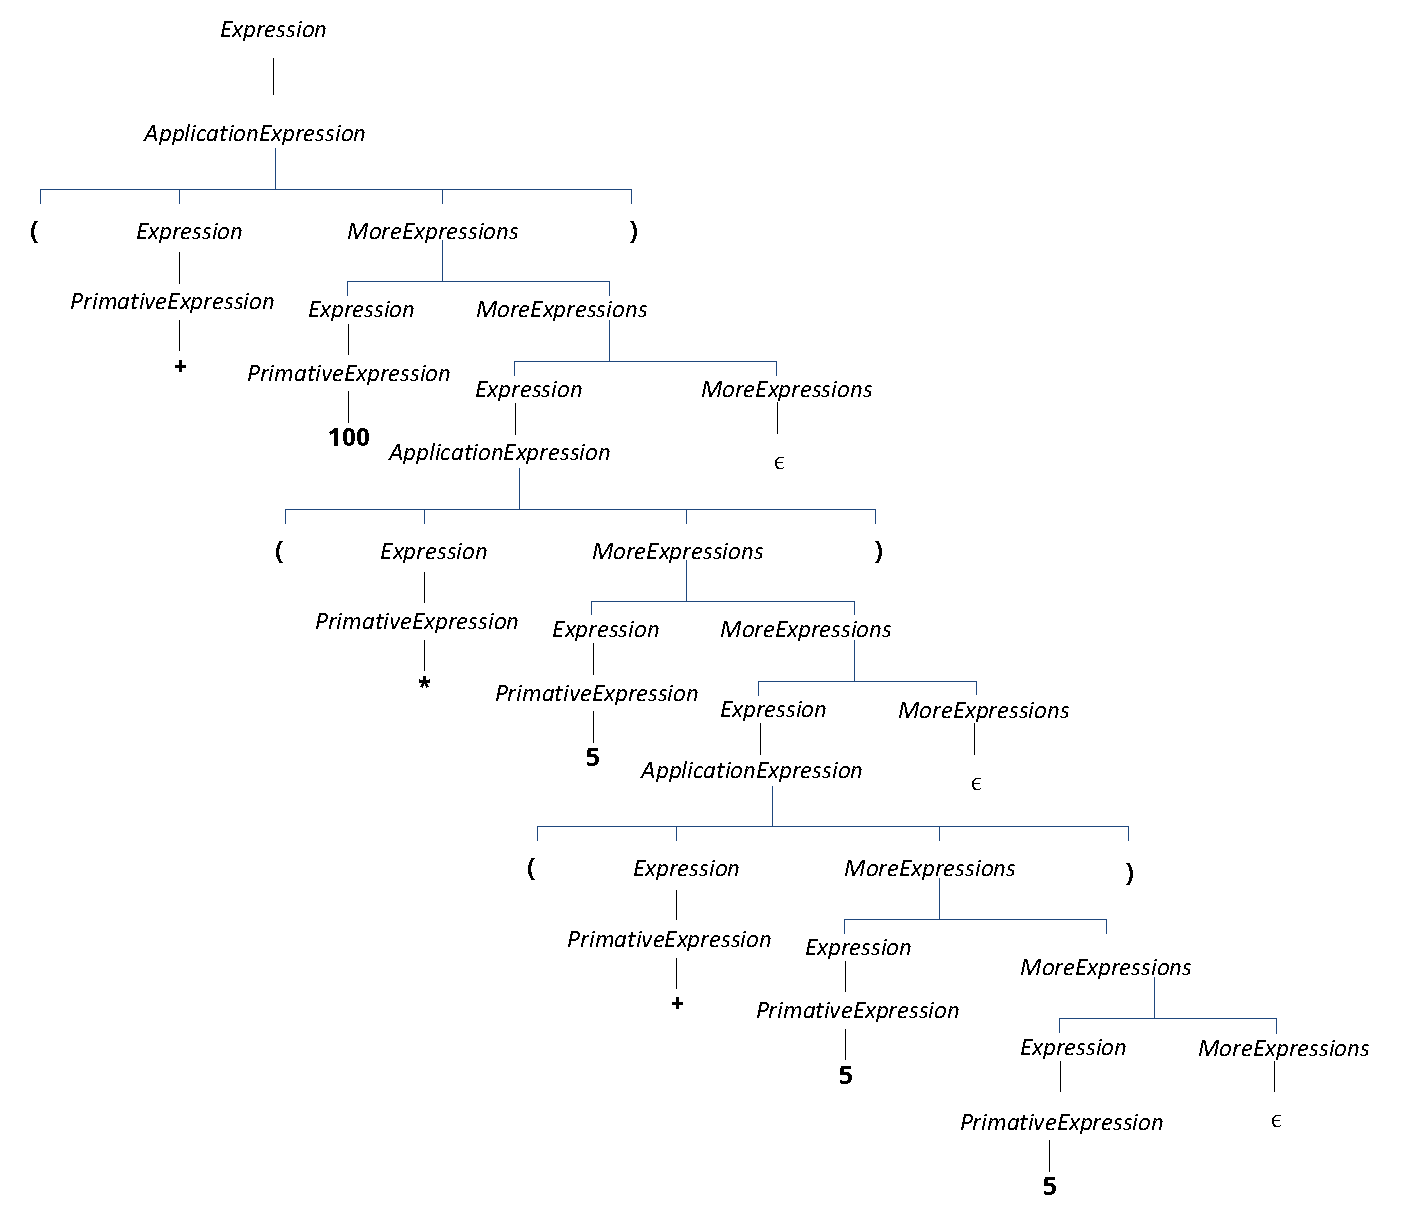
\includegraphics[width=6.0in]{figures/exercise-big-expression.pdf}
\end{center}
The main subexpressions are evaluated as shown below to produce the final value of \tb{\schemeresult|150|}.
\begin{center}
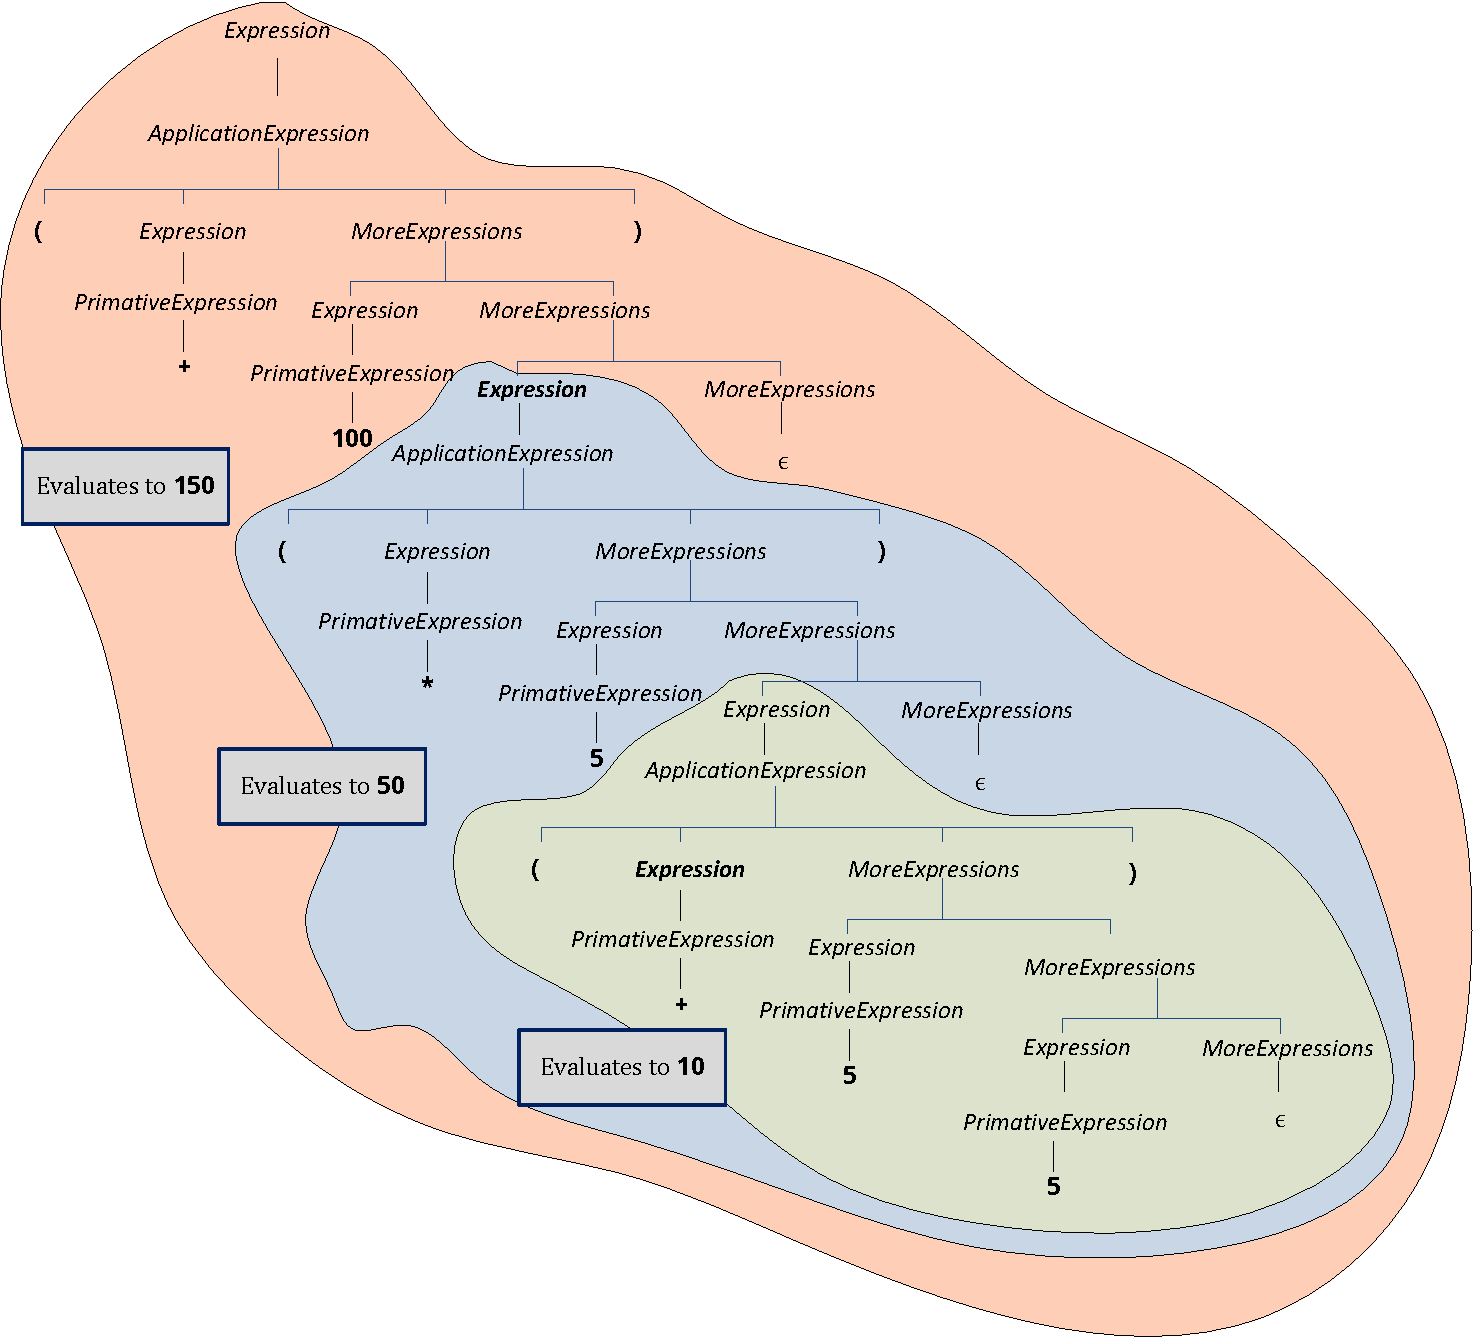
\includegraphics[width=6.0in]{figures/exercise-big-expression-with-eval.pdf}
\end{center}
}
\end{exercise}
\afterex

\beforeex
\begin{exercise}
Predict how each of the following Scheme expressions is evaluated.  After making your prediction, try evaluating the expression in DrRacket.  If the result is different from your prediction, explain why the Scheme interpreter evaluates the expression as it does.
\begin{subexerciselist}
\item \scheme|1120|
\solution{\tb{\schemeresult|1120|}}
\item \scheme|(+ 1120)|
\solution{\tb{\schemeresult|1120|}}
\item \scheme|(+ (+ 10 20) (* 2 0))|
\solution{\tb{\schemeresult|30|}}
\item \scheme|(= (+ 10 20) (* 15 (+ 5 5)))|
\solution{\tb{\schemeresult|#f|}
\par
The \scheme|#f| symbol represents the Boolean value \emph{false}.  Since the two operand expressions for the \scheme|=| have different values, the expression evaluates to \schemeresult|#f|.
}

%\item \scheme|(zero? (- 15 (+ 5 5 (+ 2 3))))|
%\solution{\tb{\schemeresult|#t|}
%\par
%The \scheme|#t| symbol represents the Boolean value \emph{true}.
%}
\item \scheme|+|
\solution{\tb{\schemeresult|#<procedure:+>|}
\par
The symbol \scheme|+| is a primitive expression that is the built-in procedure for addition.
}
\item \scheme|(+ + <)|
\solution{\bugresult{+: expects type $<$number$>$ as 1st argument, given: \#$<$procedure:+$>$; other arguments were: \#$<$procedure:$<$$>$}
\par
The interpreter produces an error since the \scheme|+| procedure is only defined for operands that are numbers.  Since the value of the first argument is a procedure, there is a type error.}
\end{subexerciselist}
\end{exercise}
\afterex

\beforeex
\begin{exercise}
For each question, construct a Scheme expression and evaluate it in DrRacket.
\begin{subexerciselist}
\item How many seconds are there in a year?
\solution{For non-leap years, there are 365 days in a year, 24 hours in a day, 60 minutes in an hour, and 60 seconds in a minute:
\scheme|(* 60 60 24 365)|
}
\item For how many seconds have you been alive?
\solution{The first number (e.g., \scheme|20| here) is the number of years you have been alive: \scheme|(* 20 60 60 24 365)|
}
\item For what fraction of your life have you been in school?
\solution{Let's assume you are 20 years old and you've been in school for 15 years and in the United States it is typical to have 180 school days in a year, and that each school day is 7 hours long.  Then, we can compute the fraction of your life spent in school by dividing the number of hours spent in school by the number of hours lived: \scheme|(/ (* 15 180 7) (* 20 365 24))|.  This evaluates to \schemeresult|63/584|.  Note that math in Scheme is exact, and it is represented as a rational number.  A more useful result is to convert it to a decimal number using the \scheme|exact->inexact| procedure:
\begin{code}
\scheme|> (exact->inexact (/ (* 15 180 7) (* 20 365 24)))|\\
\tb{\schemeresult|0.10787671232876712|}
\end{code}
Your answer, of course, will vary depending on how old you are, how many years you've spent in school, and the length of your school year and day.
}
\end{subexerciselist}
\end{exercise}
\afterex

\beforeex
\begin{exercise}
Construct a Scheme expression to calculate the distance in inches that light travels during the time it takes the processor in your computer to execute one cycle.  (A meter is defined as the distance light travels in $1/299792458^{th}$ of a second in a vacuum.  Hence, light travels at $299,792,458$ meters per second.  Your processor speed is probably given in \emph{gigahertz} (GHz), which are 1,000,000,000 hertz.  One hertz means once per second, so 1~GHz means the processor executes 1,000,000,000 cycles per second.  On a Windows machine, you can find the speed of your processor by opening the \keyword{Control Panel} (select it from the \keyword{Start} menu) and selecting \keyword{System}.  Note that Scheme performs calculations exactly, so the result will be displayed as a fraction.  To see a more useful answer, use \scheme|(exact->inexact |\nonterminal{Expression}\scheme|)| to convert the value of the expression to a decimal representation.)

\solution{
My computer is 2.33~GHz.  Hence, one cycle takes \scheme|(/ 1 2330000000)| seconds.  Light travels \scheme|299792458| meters per second.  So, in the time the processor executes a single cycle, light travels
\begin{code}
\scheme|> (exact->inexact (* 299792458 (/ 1 2330000000)))|\\
\tb{\schemeresult|0.12866629098712445|}
\end{code}
meters.  This is equivalent to
\begin{code}
\scheme|> (exact->inexact (/ (* 100 (* 299792458 (/ 1 2330000000))) 2.54))|\\
\tb{\schemeresult|5.065602007367104|}
\end{code}
inches.  This should give you some sense of how close the processor speed is to reaching physical limits.
}

\end{exercise}
\afterex

\end{schemeregion}


\section{Definitions}\label{sec:definitions}\index{general}{definition}\index{general}{abstraction}

Scheme provides a simple, yet powerful, mechanism for abstraction.  A definition introduces a new name and gives it a value:

\begin{bnfgrammarm}{Definition}
\bnfrule{Definition}{\scheme|(define| \terminal{\emph{Name}} \nonterminal{Expression}\scheme|)|}
\end{bnfgrammarm}

After a definition, the \terminal{\emph Name} in the definition is now associated with the value of the expression in the definition.  A definition is not an expression since it does not evaluate to a value.

\index{general}{name}A name can be any sequence of letters, digits, and special characters (such as \scheme|-|, \scheme|>|, \scheme|?|, and \scheme|!|) that starts with a letter or special character.  Examples of valid names include \scheme|a|, \scheme|Ada|, \scheme|Augusta-Ada|, \scheme|gold49|, \scheme|!yuck|, and \scheme|yikes!\%@\#|.  We don't recommend using some of these names in your programs, however!  A good programmer will pick names that are easy to read, pronounce, and remember, and that are not easily confused with other names.

After a name has been bound to a value by a definition, that name may be used in an expression:
\begin{bnfgrammarm}{NameExpression}
\bnfrule{Expression}{\nonterminal{NameExpression}}
\bnfrule{NameExpression}{\terminal{\emph{Name}}}
\end{bnfgrammarm}
The value of a \nonterminal{NameExpression} is the value associated with the \terminal{\emph{Name}}.  (Alert readers should be worried that we need a more precise definition of the meaning of definitions to know what it means for a value to be associated with a name.  This informal notion will serve us well for now, but we will need a more precise explanation of the meaning of a definition in Chapter~\ref{ch:state}.)

%% \clearpage %%!
Below we define \scheme|speed-of-light| to be the speed of light in meters per second, define \scheme|seconds-per-hour| to be the number of seconds in an hour, and use them to calculate the speed of light in kilometers per hour:
%\footnote{Text after a \scheme|%| in Scheme code is a \emph{comment}.  The Scheme interpreter will ignore any text after the \scheme|%| until the end of the line.}
\begin{code}
\scheme|> (define speed-of-light 299792458)|\\
\scheme|> speed-of-light| \\
\tb{\schemeresult|299792458|} \\
\scheme|> (define seconds-per-hour (* 60 60))| \\
\scheme|> (/ (* speed-of-light seconds-per-hour) 1000)| \\
\tb{\schemeresult|1079252848 4/5|} %!!
\end{code}

\section{Procedures}\label{sec:procedures}\index{general}{procedure}

In Chapter~\ref{ch:intro} we defined a procedure as a description of a process.  Scheme provides a way to define procedures that take inputs, carry out a sequence of actions, and produce an output.  Section~\ref{built-in-procs} introduced some of Scheme's primitive procedures.  To construct complex programs, however, we need to be able to create our own procedures.  

Procedures are similar to mathematical functions in that they provide a mapping between inputs and outputs, but they differ from mathematical functions in two important ways:
\begin{descriptionlist}
\item[{\bf State.}] In addition to producing an output, a procedure may access and modify state.  This means that even when the same procedure is applied to the same inputs, the output produced may vary.  Because mathematical functions do not have external state, when the same function is applied to the same inputs it always produces the same result.  State makes procedures much harder to reason about.  %In particular, it breaks the substitution model of evaluation we introduce in the next section.  
We will ignore this issue until Chapter~\ref{ch:state}, and focus until then only on procedures that do not involve any state.\index{general}{state}
\item[{\bf Resources.}] Unlike an ideal mathematical function, which provides an instantaneous and free mapping between inputs and outputs, a procedure requires resources to execute before the output is produced.  The most important resources are \emph{space} (memory) and \emph{time}.  A procedure may need space to keep track of intermediate results while it is executing.  Each step of a procedure requires some time to execute.  Predicting how long a procedure will take to execute and finding the fastest procedure possible for solving some problem are core problems in computer science.  We consider this throughout this book, and in particular in Chapter~\ref{ch:cost}.  %Even knowing if a procedure will finish is a challenging problem.  In Chapter~\ref{ch:computability} we will see that it is impossible to solve in general.
\end{descriptionlist}

For the rest of this chapter, we view procedures as idealized mathematical functions: we consider only procedures that involve no state and do not worry about the resources required to execute our procedures.

\subsection{Making Procedures}\index{general}{procedure}

Scheme provides a general mechanism for making a procedure:\index{general}{lambda}
\begin{schemeregion}
\begin{bnfgrammarm}{ProcedureExpression}
\bnfrule{Expression}{\nonterminal{ProcedureExpression}}
\bnfrule{ProcedureExpression}{\scheme|(lambda (|\nonterminal{Parameters}\scheme|)| \nonterminal{Expression}\scheme|)|}
\bnfrule{Parameters}{$\epsilon$ $\mid$ \terminal{\emph{Name}} \nonterminal{Parameters}}
\end{bnfgrammarm}
\end{schemeregion}
Evaluating a \nonterminal{ProcedureExpression} produces a procedure that takes as inputs the \nonterminal{Parameters} following the \scheme|lambda|.
%\cut{\footnote{Scheme uses \scheme|lambda| to make a procedure because it is based on LISP which is based on Lambda Calculus\cut{(see Chapter~\ref{ch:alternatemodels})}.}} 
The \scheme|lambda| special form means ``make a procedure''.  The body of the resulting procedure is the \nonterminal{Expression}, which is not evaluated until the procedure is applied.

A \nonterminal{ProcedureExpression} can replace an \nonterminal{Expression}.  This means anywhere an \emph{Expression} is used we can create a new procedure.  This is very powerful since it means we can use procedures as inputs to other procedures and create procedures that return new procedures as their output!  

Here are some example procedures:
\begin{schemeregion}
\begin{descriptionlist}
\item[\scheme|(lambda (x) (* x x))|] \forcenl Procedure that takes one input, and produces the square of the input value as its output.
\item[\scheme|(lambda (a b) (+ a b))|] \forcenl Procedure that takes two inputs, and produces the sum of the input values as its output.
\item[\scheme|(lambda () 0)|] \forcenl Procedure that takes no inputs, and produces \tb{\schemeresult{0}} as its output.  The result of applying this procedure to any argument is always \tb{\schemeresult{0}}.
\item[\scheme|(lambda (a) (lambda (b) (+ a b)))|] \forcenl Procedure that takes one input (\scheme|a|), and produces as its output a procedure that takes one input and produces the sum of \scheme|a| and that input as its output.  This is an example of a \definition{higher-order procedure}.  Higher-order procedures produce procedures as their output or take procedures as their arguments.  This can be confusing, but is also very powerful.
\end{descriptionlist}
\end{schemeregion}

\subsection{Substitution Model of Evaluation}\label{sec:substitution-model}

For a procedure to be useful, we need to apply it.  In Section~\ref{sec:application}, we saw the syntax and evaluation rule for an \nonterminal{ApplicationExpression} when the procedure to be applied is a primitive procedure.  The syntax for applying a constructed procedure is identical to the syntax for applying a primitive procedure:
\begin{schemeregion}
\begin{bnfgrammarm}{ApplicationExpression}
\bnfrule{Expression}{\nonterminal{ApplicationExpression}}
\bnfrule{ApplicationExpression}{\scheme|(|\nonterminal{Expression} \nonterminal{MoreExpressions}\scheme|)|}
\bnfrule{MoreExpressions}{$\epsilon$ $\mid$ \nonterminal{Expression} \nonterminal{MoreExpressions}}
\end{bnfgrammarm}
\end{schemeregion}

To understand how constructed procedures are evaluated, we need a new evaluation rule.  In this case, the first \nonterminal{Expression} evaluates to a procedure that was created using a \nonterminal{ProcedureExpression}, so the \nonterminal{ApplicationExpression} becomes: 
\begin{schemeregion}
\begin{bnfgrammarm}{ApplicationExpression}
\bnfruleplain{ApplicationExpression}{\\ \hspace*{6em}\scheme|(|\underline{\scheme|(lambda (|\nonterminal{Parameters}\scheme|)|\nonterminal{Expression}\scheme|)|} \nonterminal{MoreExpressions}\scheme|)|}
\end{bnfgrammarm}
\end{schemeregion} (The underlined part is the replacement for the \nonterminal{ProcedureExpression}.)

\index{general}{application}
To evaluate the application, first evaluate the \nonterminal{MoreExpressions} in the application expression.  These expressions are known as the \emph{operands} of the application.  The resulting values are the inputs to the procedure.  There must be exactly one expression in the \nonterminal{MoreExpressions} corresponding to each name in the parameters list.  Next, associate the names in the \nonterminal{Parameters} list with the corresponding operand values.  Finally, evaluate the expression that is the body of the procedure.  Whenever any parameter name is used inside the body expression, the name evaluates to the value of the corresponding input that is associated with that name.

\begin{examplenobar}{Square}\index{general}{square}
\begin{schemeregion}
Consider evaluating the following expression: %, which apples the squaring procedure to \scheme|2|:
\begin{schemedisplay}
((lambda (x) (* x x)) 2)
\end{schemedisplay}
It is an \nonterminal{ApplicationExpression} where the first subexpression is the \nonterminal{ProcedureExpression}, \scheme|(lambda (x) (* x x))|.  To evaluate the application, we evaluate all the subexpressions and apply the value of the first subexpression to the values of the remaining subexpressions.  The first subexpression evaluates to a procedure that takes one parameter named \scheme|x| and has the expression body \scheme|(* x x)|.  There is one operand expression, the primitive \scheme|2|, that evaluates to \tb{\schemeresult|2|}.  

To evaluate the application we bind the first parameter, \scheme|x|, to the value of the first operand, \tb{\schemeresult|2|}, and evaluate the procedure body, \scheme|(* x x)|.  After substituting the parameter values, we have \scheme|(* 2 2)|.  This is an application of the primitive multiplication procedure.  Evaluating the application results in the value \tb{\schemeresult|4|}.  

The procedure in our example, \scheme|(lambda (x) (* x x))|, is a procedure that takes a number as input and as output produces the square of that number.  We can use the definition mechanism (from Section~\ref{sec:definitions}) to give this procedure a name so we can reuse it:
\begin{schemedisplay}
(define square (lambda (x) (* x x)))
\end{schemedisplay}
This defines the name \scheme|square| as the procedure.  After this, we can apply \scheme|square| to any number:
\begin{code}
\scheme|> (square 2)|\\
\tb{\schemeresult|4|}\\
\scheme|> (square 1/4)|\\
\tb{\schemeresult|1/16|} \\
\scheme|> (square (square 2))|\\
\tb{\schemeresult|16|}\\
\end{code}
\end{schemeregion}
\end{examplenobar}

\begin{schemeregion}
\begin{example}{Make adder}
The expression
\begin{schemedisplay}
((lambda (a) 
   (lambda (b) (+ a b))) 
 3)
\end{schemedisplay}
evaluates to a procedure that adds \scheme|3| to its input.  Applying that procedure to \scheme|4|,
\begin{schemedisplay}
(((lambda (a) (lambda (b) (+ a b))) 3) 
 4)
\end{schemedisplay}
evaluates to \tb{\schemeresult|7|}.  By using \scheme|define|, we can give these procedures sensible names:
\begin{schemedisplay}
(define make-adder 
  (lambda (a)
    (lambda (b) (+ a b))))
\end{schemedisplay}
Then, \scheme|(define add-three (make-adder 3))| defines \scheme|add-three| as a procedure that takes one parameter and outputs the value of that parameter plus \scheme|3|.
\end{example}
\end{schemeregion}

\shortsection{Abbreviated Procedure Definitions} Since we commonly define new procedures, Scheme provides a condensed notation for defining a procedure\footnote{The condensed notation also includes a begin expression, which is a special form.  We will not need the begin expression until we start dealing with procedures that have side effects.  We describe the \scheme|begin| special form in Chapter~\ref{ch:state}.}:

\begin{schemeregion}
\begin{bnfgrammarm}{Definition}
\bnfrule{Definition}{\scheme|(define (|\terminal{\emph{Name}} \nonterminal{Parameters}\scheme|)| \nonterminal{Expression}\scheme|)|}
\end{bnfgrammarm}

This incorporates the \scheme|lambda| invisibly into the definition, but means exactly the same thing.  For example,
\begin{schemedisplay}
(define square (lambda (x) (* x x)))
\end{schemedisplay}
can be written equivalently as:
\begin{schemedisplay}
(define (square x) (* x x))
\end{schemedisplay}

\beforeex
\begin{exercise}
Define a procedure, \scheme|cube|, that takes one number as input and produces as output the cube of that number.
\solution{
\begin{schemedisplay}
(define cube (lambda (x) (* x x x)))
\end{schemedisplay}
or:
\begin{schemedisplay}
(define (cube x) (* x x x))
\end{schemedisplay}
}
\end{exercise}
\afterex

\beforeex
\begin{exercise}
Define a procedure, \scheme|compute-cost|, that takes as input two numbers, the first represents that price of an item, and the second represents the sales tax rate.  The output should be the total cost, which is computed as the price of the item plus the sales tax on the item, which is its price times the sales tax rate.  For example, \scheme|(compute-cost 13 0.05)| should evaluate to \tb{\schemeresult|13.65|}.
\solution{
\begin{schemedisplay}
(define compute-cost 
   (lambda (price rate)
      (+ price (* price rate))))
\end{schemedisplay}      
Another approach:
\begin{schemedisplay}
(define (compute-cost price rate)
   (* price (+ 1 rate)))
\end{schemedisplay}
}
\end{exercise}
\afterex
\end{schemeregion}

%\TODO{Add more exercises here}

\section{Decisions}\label{sec:decisions}\label{sec:if}

To make more useful procedures, we need the actions taken to depend on the input values.  For example, we may want a procedure that takes two numbers as inputs and evaluates to the greater of the two inputs.  To define such a procedure we need a way of making a decision.  The \nonterminal{IfExpression} expression provides a way of using the result of one expression to select which of two possible expressions to evaluate:
\begin{schemeregion}
\begin{bnfgrammarm}{IfExpression}
\bnfrule{Expression}{\nonterminal{IfExpression}}
\bnfrule{IfExpression}{\scheme|(if |\=\nonterminal{Expression$_{\rm Predicate}$}}
\> \> \> \nonterminal{Expression$_{\rm Consequent}$}\\
\> \> \> \nonterminal{Expression$_{\rm Alternate}$}\scheme|)|\\
\end{bnfgrammarm}
\end{schemeregion}
The \nonterminal{IfExpression} replacement has three \nonterminal{Expression} terms.  For clarity, we give each of them names as denoted by the Predicate, Consequent, and Alternate subscripts.  To evaluate an \nonterminal{IfExpression}, first evaluate the predicate expression, \nonterminal{Expression$_{\rm Predicate}$}.  If it evaluates to any non-false value, the value of the \nonterminal{IfExpression} is the value of \nonterminal{Expression$_{\rm Consequent}$}, the consequent expression, and the alternate expression is not evaluated at all.  If the predicate expression evaluates to false, the value of the \nonterminal{IfExpression} is the value of \nonterminal{Expression$_{\rm Alternate}$}, the alternate expression, and the consequent expression is not evaluated at all.  

The predicate expression determines which of the two following expressions is evaluated to produce the value of the \nonterminal{IfExpression}.  If the value of the predicate is \emph{anything} other than \tb{\schemeresult|false|}, the consequent expression is used.  For example, if the predicate evaluates to \tb{\schemeresult|true|}, to a number, or to a procedure the consequent expression is evaluated.

The if expression is a \definition{special form}.  This means that although it looks syntactically identical to an application (that is, it could be an application of a procedure named \scheme|if|), it is not evaluated as a normal application would be.  Instead, we have a special evaluation rule for if expressions.  The reason a special evaluation rule is needed is because we do not want all the subexpressions to be evaluated.  With the normal application rule, all the subexpressions are evaluated first, and then the procedure resulting from the first subexpression is applied to the values resulting from the others.  With the if special form evaluation rule, the predicate expression is always evaluated first and only one of the following subexpressions is evaluated depending on the result of evaluating the predicate expression.  

\begin{schemeregion}
This means an if expression can evaluate to a value even if evaluating one of its subexpressions would produce an error.  For example,
\begin{schemedisplay}
(if (> 3 4) (* + +) 7)
\end{schemedisplay}
evaluates to \tb{\schemeresult|7|} even though evaluating the subexpression \scheme|(* + +)| would produce an error.  Because of the special evaluation rule for if expressions, the consequent expression is never evaluated. 
\end{schemeregion}

\begin{example}{Bigger}\label{example:bigger}
\begin{schemeregion}
Now that we have procedures, decisions, and definitions, we can understand the \scheme|bigger| procedure from the beginning of the chapter.  The definition,
\begin{schemedisplay}
(define (bigger a b) (if (> a b) a b))
\end{schemedisplay}
is a condensed procedure definition.  It is equivalent to:
\begin{schemedisplay}
(define bigger (lambda (a b) (if (> a b) a b)))
\end{schemedisplay}
This defines the name \scheme|bigger| as the value of evaluating the procedure expression \scheme|(lambda (a b) (if (> a b) a b))|.  This is a procedure that takes two inputs, named \scheme|a| and \scheme|b|.   Its body is an if expression with predicate expression \scheme|(> a b)|.  The predicate expression compares the value that is bound to the first parameter, \scheme|a|, with the value that is bound to the second parameter, \scheme|b|, and evaluates to \tb{\schemeresult|true|} if the value of the first parameter is greater, and \tb{\schemeresult|false|} otherwise.  According to the evaluation rule for an if expression, when the predicate evaluates to any non-false value (in this case, \tb{\schemeresult|true|}), the value of the if expression is the value of the consequent expression, \scheme|a|.  When the predicate evaluates to \tb{\schemeresult|false|}, the value of the if expression is the value of the alternate expression, \scheme|b|.  Hence, our \scheme|bigger| procedure takes two numbers as inputs and produces as output the greater of the two inputs.
\end{schemeregion}
\end{example}

\begin{schemeregion}
\beforeex
\begin{exercise}
Follow the evaluation rules to evaluate the Scheme expression: 
\begin{schemedisplay}
(bigger 3 4)
\end{schemedisplay}
where \scheme|bigger| is the procedure defined above.  (It is very tedious to follow all of the steps (that's why we normally rely on computers to do it!), but worth doing once to make sure you understand the evaluation rules.)
\LATER{solution}
\end{exercise}
\afterex

\beforeex
\begin{exercise}
Define a procedure, \scheme|xor|, that implements the logical ex\-clu\-sive-or operation.  \LATER{described in Section~\ref{sec:composingoperations}.}  The \scheme|xor| function takes two inputs, and outputs \tb{\schemeresult|true|} if exactly one of those outputs has a true value.  Otherwise, it outputs \tb{\schemeresult|false|}.  For example, \scheme|(xor true true)| should evaluate to \tb{\schemeresult|false|} and \scheme|(xor (< 3 5) (= 8 8))| should evaluate to \tb{\schemeresult|true|}.
\solution{
There are many possible ways to define \scheme|xor|.  Here are two possibilities:
\begin{schemedisplay}
(define (xor a b)
   (if a (not b) b))
\end{schemedisplay}

\begin{schemedisplay}
(define (xor a b)
   (or (and a (not b)) (and (not a) b)))
\end{schemedisplay}
}
\end{exercise}
\afterex

\beforeex
\begin{exercise}
Define a procedure, \scheme|absvalue|, that takes a number as input and produces the absolute value of that number as its output.  For example, \scheme|(absvalue 3)| should evaluate to \tb{\schemeresult|3|} and \scheme|(absvalue -150)| should evaluate to \tb{\schemeresult|150|}.
\solution{
\begin{schemedisplay}
(define (absvalue v)
   (if (< v 0) (- v) v))
\end{schemedisplay}
Note that Scheme provides a built-in function \scheme|abs| that implements the absolute value function.  Hence, the easiest way to define \scheme|absvalue| would be,
\begin{schemedisplay}
(define absvalue abs)
\end{schemedisplay}
}
\end{exercise}
\afterex

\beforeex
\begin{exercise}\bluestar
Define a procedure, \scheme|bigger-magnitude|, that takes two inputs, and outputs the value of the input with the greater magnitude (that is, absolute distance from zero). For example,
\scheme|(bigger-magnitude 5 -7)|
should evaluate to \tb{\schemeresult|-7|}, and
\scheme|(bigger-magnitude 9 -3)|
should evaluate to \tb{\schemeresult|9|}.
\solution{
We use the \scheme|absvalue| procedure defined in the previous exercise:
\begin{schemedisplay}
(define (bigger-magnitude a b)
   (if (> (absvalue a) (absvalue b)) a b))
\end{schemedisplay}
}
\end{exercise}
\afterex

\beforeex
\begin{exercise}\bluestar\label{exer:biggest}
Define a procedure, \scheme|biggest|, that takes three inputs, and produces as output the maximum value of the three inputs.  For example, 
\scheme|(biggest 5 7 3)| should evaluate to \tb{\schemeresult|7|}.  Find at least two different ways to define \scheme|biggest|, one using \scheme|bigger|, and one without using it.
\solution{
Our first solution uses the \scheme|bigger| procedure from Example~\ref{example:bigger}:
\begin{schemedisplay}
(define (biggest a b c)
   (bigger (bigger a b) c))
\end{schemedisplay}
Another approach is to define an if expression:
\begin{schemedisplay}
(define (biggest a b c)
   (if (> a b)
       (if (> a c) a c)
       (if (> b c) b c)))
\end{schemedisplay}
We prefer the first version since it is shorter and easier to understand.  This is a simple illustration of the advantages of building up more complex procedures by combining simple ones.
}
\end{exercise}
\afterex

\end{schemeregion}

\section{Evaluation Rules}\label{sec:rules}\index{general}{rules of evaluation}

Here we summarize the grammar rules and evaluation rules.  Since each grammar rule has an associated evaluation rule, we can determine the meaning of any grammatical Scheme fragment by combining the evaluation rules corresponding to the grammar rules followed to derive that fragment.

\groupcontent{
\bnfruleg{Program}{$\epsilon$ $\mid$ \nonterminal{ProgramElement} \nonterminal{Program}}
\bnfruleg{ProgramElement}{\nonterminal{Expression} $\mid$ \nonterminal{Definition}}
\evalrule{A program is a sequence of expressions and definitions.}
}

\groupcontent{
\bnfruleg{Definition}{\scheme|(define| \terminal{\emph{Name}} \nonterminal{Expression}\scheme|)|} 
\evalrule{A definition evaluates the expression, and associates the value of the expression with the name.}
}

\groupcontent{\bnfruleg{Definition}{\scheme|(define (|\terminal{\emph{Name}} \nonterminal{Parameters}\scheme|)| \nonterminal{Expression}\scheme|)|}
\evalrule{Abbreviation for\\\hspace*{0.2in} \scheme|(define| \terminal{\emph{Name}} \scheme|(lambda| \nonterminal{Parameters}\scheme|)| \nonterminal{Expression}\scheme|)|}
}

\groupcontent{
\bnfruleg{Expression}{\nonterminal{PrimitiveExpression} 
			      $\mid$ \nonterminal{NameExpression} \\
			    	$\mid$ \nonterminal{ApplicationExpression} \\
			    	$\mid$ \nonterminal{ProcedureExpression}
			    	$\mid$ \nonterminal{IfExpression}}
\evalrule{The value of the expression is the value of the replacement expression.}
}

\groupcontent{
\bnfruleg{PrimitiveExpression}{\terminal{\emph{Number}} $\mid$ \scheme|true| $\mid$ \scheme|false| $\mid$ \emph{primitive procedure}}
\evalrule{\bold{Evaluation Rule 1: Primitives.}  A primitive expression evaluates to its pre-defined value.}
}

\groupcontent{
\bnfruleg{NameExpression}{\terminal{\emph{Name}}}
\evalrule{\bold{Evaluation Rule 2: Names.}  A name evaluates to the value associated with that name.}
}

\groupcontent{
\bnfruleg{ApplicationExpression}{\scheme|(|\nonterminal{Expression} \nonterminal{MoreExpressions}\scheme|)|}
\evalrule{\bold{Evaluation Rule 3: Application.}  To evaluate an application expression: 
\begin{enumerate}[\bfseries a.]
\item \bold{Evaluate} all the subexpressions; 
\item Then, \bold{apply} the value of the first subexpression to the values of the remaining subexpressions.
\end{enumerate}}}

\groupcontent{
\bnfruleg{MoreExpressions}{$\epsilon$ $\mid$ \nonterminal{Expression} \nonterminal{MoreExpressions}}
\bnfruleg{ProcedureExpression}{\scheme|(lambda (|\nonterminal{Parameters}\scheme|)| \nonterminal{Expression}\scheme|)|}
\bnfruleg{Parameters}{$\epsilon$ $\mid$ \terminal{\emph{Name}} \nonterminal{Parameters}}
\evalrule{\bold{Evaluation Rule 4: Lambda.}  Lambda expressions evaluate to a procedure that takes the given parameters and has the expression as its body.}
}

\groupcontent{
\bnfruleg{IfExpression}{\scheme|(if| \nonterminal{Expression$_{\rm Predicate}$}\\\hspace*{0.2in}\nonterminal{Expression$_{\rm Consequent}$}\\\hspace*{0.2in}\nonterminal{Expression$_{\rm Alternate}$}\scheme|)|}
\evalrule{\bold{Evaluation Rule 5: If.}  To evaluate an if expression, (a) evaluate the predicate expression; then, (b) if the value of the predicate expression is a false value then the value of the if expression is the value of the alternate expression; otherwise, the value of the if expression is the value of the consequent expression.}
}

\vspace*{1.5ex}

\groupcontent{
The evaluation rule for an application (Rule 3b) uses \bold{apply} to perform the application.  Apply is defined by the two application rules:
\vspace*{0.5ex}

\begin{descriptionlist}
\item[\bold{Application Rule 1: Primitives.}] \forcenl To apply a primitive procedure, just do it.
\item[\bold{Application Rule 2: Constructed Procedures.}] \forcenl To apply a constructed procedure, \bold{evaluate} the body of the procedure with each parameter name bound to the corresponding input expression value.
\end{descriptionlist}
}

Application Rule 2 uses the evaluation rules to \bold{evaluate} the expression.  Thus, the evaluation rules are defined using the application rules, which are defined using the evaluation rules!  This appears to be a circular definition, but as with the grammar examples, it has a base case.  Some expressions evaluate without using the application rules (e.g., primitive expressions, name expressions), and some applications can be performed without using the evaluation rules (when the procedure to apply is a primitive).  Hence, the process of evaluating an expression will sometimes finish and when it does we end with the value of the expression.\footnote{This does not guarantee that evaluation \emph{always} finishes, however!  The next chapter includes some examples where evaluation never finishes.}

\section{Summary}

At this point, we have covered enough of Scheme to write useful programs (even if the programs we have seen so far seem rather dull).  In fact (as we show in Chapter~\ref{ch:universal}), we have covered enough to express \emph{every} possible computation!  We just need to combine these constructs in more complex ways to perform more interesting computations.  The next chapter (and much of the rest of this book), focuses on ways to combine the constructs for making procedures, making decisions, and applying procedures in more powerful ways.

